\documentclass[12pt,a4paper]{article}

\usepackage[spanish,es-tabla]{babel}
\usepackage[T1]{fontenc}
\usepackage[utf8]{inputenc}
\usepackage{lmodern}
\usepackage[a4paper,margin=2.5cm]{geometry}
\usepackage{setspace}
\usepackage{parskip}
\usepackage{hyperref}
\usepackage{graphicx}
\usepackage{float}
\usepackage{enumitem}
\usepackage{xcolor}

\hypersetup{
    colorlinks=true,
    linkcolor=blue,
    urlcolor=blue,
    pdftitle={Manual de Usuario Global de Instalaciones},
    pdfauthor={OpenAI Codex}
}

\setstretch{1.1}
\setlist[itemize]{topsep=4pt,itemsep=2pt}
\setlist[enumerate]{topsep=4pt,itemsep=2pt}

\newcommand{\placeholderimage}[2]{
    \begin{figure}[H]
        \centering
        \fbox{\parbox[c][6cm][c]{0.88\textwidth}{
            \centering
            \textbf{#1}\\[0.4cm]
            #2
        }}
        \caption{#2}
    \end{figure}
}

\newcommand{\manualimage}[2]{
    \IfFileExists{#1}{
        \begin{figure}[H]
            \centering
            \includegraphics[width=0.9\textwidth]{#1}
            \caption{#2}
        \end{figure}
    }{
        \placeholderimage{#1}{#2}
    }
}

\newcommand{\manualimagesized}[4]{
    \IfFileExists{#1}{
        \begin{figure}[H]
            \centering
            \includegraphics[width=#3,height=#4,keepaspectratio]{#1}
            \caption{#2}
        \end{figure}
    }{
        \placeholderimage{#1}{#2}
    }
}

\newcommand{\manualtripleimage}[4]{
    \IfFileExists{#1}{
        \begin{figure}[H]
            \centering
            \includegraphics[width=0.31\textwidth]{#1}\hfill
            \includegraphics[width=0.31\textwidth]{#2}\hfill
            \includegraphics[width=0.31\textwidth]{#3}
            \caption{#4}
        \end{figure}
    }{
        \placeholderimage{#1 / #2 / #3}{#4}
    }
}

\newcommand{\manualtripleimagelabeled}[7]{
    \IfFileExists{#1}{
        \begin{figure}[H]
            \centering
            \begin{minipage}[t]{0.31\textwidth}
                \centering
                \includegraphics[width=\textwidth]{#1}\\[0.15cm]
                \footnotesize #2
            \end{minipage}\hfill
            \begin{minipage}[t]{0.31\textwidth}
                \centering
                \includegraphics[width=\textwidth]{#3}\\[0.15cm]
                \footnotesize #4
            \end{minipage}\hfill
            \begin{minipage}[t]{0.31\textwidth}
                \centering
                \includegraphics[width=\textwidth]{#5}\\[0.15cm]
                \footnotesize #6
            \end{minipage}
            \caption{#7}
        \end{figure}
    }{
        \placeholderimage{#1 / #3 / #5}{#7}
    }
}

\newcommand{\manualdoubleimagelabeled}[5]{
    \IfFileExists{#1}{
        \begin{figure}[H]
            \centering
            \begin{minipage}[t]{0.48\textwidth}
                \centering
                \includegraphics[width=\textwidth]{#1}\\[0.15cm]
                \footnotesize #2
            \end{minipage}\hfill
            \begin{minipage}[t]{0.48\textwidth}
                \centering
                \includegraphics[width=\textwidth]{#3}\\[0.15cm]
                \footnotesize #4
            \end{minipage}
            \caption{#5}
        \end{figure}
    }{
        \placeholderimage{#1 / #3}{#5}
    }
}

\newcommand{\pendingtag}{\textcolor{red}{\textbf{[PENDIENTE DE CONFIRMAR EN ENTORNO REAL]}}}

\title{Manual de Usuario Global de Instalaciones}
\author{}
\date{\today}

\begin{document}

\maketitle
\tableofcontents
\newpage

\section{Finalidad del manual}

Este manual explica cómo funciona una instalación dentro de Allplan desde el punto de vista del usuario.

Se ha tomado la instalación de Agua como ejemplo, pero el funcionamiento general es común al resto de instalaciones. Lo que cambia entre unas y otras son algunos elementos concretos, ciertos nombres de layer y algunos atributos, pero la forma de trabajar es prácticamente la misma.

El objetivo de este documento es que cualquier usuario pueda entender:

\begin{itemize}
\item cómo empezar una instalación;
\item cómo dibujarla;
\item cómo editarla;
\item cómo aplicar layers y atributos;
\item cómo insertar elementos definidos, macros y soportes;
\item cómo funcionan las copias o duplicados;
\item y qué comprobaciones conviene hacer antes de finalizar.
\end{itemize}

\section{A quién va dirigido}

Este manual está pensado para usuarios que necesiten modelar instalaciones en Allplan y entender el comportamiento general de la herramienta, sin entrar en detalles de programación ni en nombres internos del sistema.

\section{Cómo se complementa este manual}

Este documento se organiza en dos grandes bloques:

\begin{enumerate}
\item El funcionamiento global de las instalaciones.
\item Las particularidades de cada instalación.
\end{enumerate}

En la primera parte se explica la lógica de uso común a todos los sistemas.

En la segunda parte se recogen las diferencias específicas de cada instalación, por ejemplo:

\begin{itemize}
\item los tipos de instalación disponibles;
\item las distribuciones admitidas;
\item los diámetros disponibles;
\item los accesorios automáticos;
\item los elementos definidos propios;
\item las limitaciones o avisos especiales;
\item y cualquier diferencia importante respecto a otras instalaciones.
\end{itemize}

De este modo, el usuario puede entender primero el funcionamiento general y después consultar, dentro del mismo manual, la unidad concreta de la instalación con la que vaya a trabajar.

Cuando aparezca el marcador \pendingtag, significa que ese dato todavía debe validarse en Allplan antes de cerrar la versión definitiva del manual.

\section{Qué partes son comunes en todas las instalaciones}

Todas las instalaciones comparten la misma lógica de trabajo:

\begin{enumerate}
\item Se selecciona el tipo de instalación.
\item Se configuran los parámetros principales en la paleta.
\item Se dibuja o edita el recorrido.
\item Se revisa la previsualización.
\item Se añaden, si hace falta, elementos definidos, macros o soportes.
\item Se aplican layers y atributos.
\item Se finaliza la creación.
\end{enumerate}

Lo que cambia entre instalaciones suele ser:

\begin{itemize}
\item el tipo de elementos disponibles;
\item los diámetros;
\item las conexiones;
\item algunos layers;
\item y algunos atributos asociados a cada sistema.
\end{itemize}

\section{Vista general del trabajo con una instalación}

El trabajo habitual con una instalación se basa en tres ideas:

\begin{itemize}
\item dibujar un recorrido;
\item enriquecer ese recorrido con información;
\item y generar el resultado final.
\end{itemize}

En la práctica, esto significa que primero se crea el trazado principal y después se añaden o ajustan el resto de elementos necesarios.

\manualimagesized{capturas/CAPTURA-01.png}{Paleta principal completa de la instalación con sus apartados visibles}{0.52\textwidth}{0.62\textheight}

\section{Flujo de trabajo recomendado}

El orden más recomendable para trabajar es este:

\begin{enumerate}
\item Elegir el tipo de instalación.
\item Elegir el tipo de tubo o sistema.
\item Definir diámetro, distribución y resto de parámetros básicos.
\item Dibujar el recorrido principal.
\item Revisar uniones, codos y bifurcaciones.
\item Aplicar layers y atributos si es necesario.
\item Insertar elementos definidos, macros o soportes.
\item Comprobar que la información esté completa.
\item Pulsar el botón de finalizar.
\end{enumerate}

Seguir este orden ayuda a evitar correcciones posteriores innecesarias.

\section{Modos principales de trabajo}

La herramienta suele trabajar con tres modos principales.

\subsection{Modo creación}

Es el modo que se utiliza para dibujar un recorrido nuevo.

En este modo el usuario va definiendo puntos y la instalación crea el trazado entre ellos.

\subsection{Modo edición}

Es el modo que se utiliza para corregir o modificar un recorrido ya dibujado.

En este modo se pueden seleccionar tramos, borrar partes, cambiar diámetros o ajustar la geometría.

\subsection{Modo extender}

Es el modo que se utiliza para continuar un recorrido ya existente sin empezar desde cero.

\section{Qué debe configurar el usuario antes de dibujar}

Antes de empezar a dibujar conviene revisar los campos principales de la paleta.

\subsection{Tipo de instalación}

Es el campo donde el usuario elige el sistema con el que va a trabajar.

En Agua, por ejemplo, puede elegir entre varias opciones como:

\begin{itemize}
\item Polietilè;
\item Multicapa;
\item Armaflex.
\end{itemize}

Este campo define qué geometría y qué comportamiento tendrá la instalación.

\manualimage{capturas/CAPTURA-02.png}{Desplegable del tipo de instalación abierto con las opciones visibles}

\subsection{Diámetro}

El diámetro condiciona:

\begin{itemize}
\item el tamaño del elemento principal;
\item las piezas de conexión compatibles;
\item y parte de los atributos asociados.
\end{itemize}

Antes de dibujar, conviene comprobar que el diámetro seleccionado es el correcto.

\subsection{Distribución}

La distribución define cómo debe comportarse la instalación dentro del sistema.

En Agua es habitual trabajar con modos como:

\begin{itemize}
\item TD;
\item IS.
\end{itemize}

La distribución puede afectar a:

\begin{itemize}
\item la forma de los elementos;
\item los atributos aplicados;
\item y el comportamiento de ciertos accesorios.
\end{itemize}

\subsection{Tipo de agua u otras variantes}

Algunas instalaciones incluyen campos adicionales para distinguir variantes internas del sistema. Si la paleta muestra este dato, conviene definirlo antes de empezar.

\subsection{Ángulos y orientación}

Si la instalación trabaja con limitación angular o con orientación definida, estos parámetros deben comprobarse al inicio para evitar tener que rehacer el recorrido más adelante.

\section{Cómo dibujar una instalación}

El dibujo de la instalación se basa en una secuencia de clics que definen el recorrido.

\subsection{Inicio del recorrido}

El usuario hace clic en el primer punto del trazado.

\subsection{Continuación del recorrido}

Cada clic adicional añade un nuevo tramo.

La herramienta va construyendo la instalación entre esos puntos y mostrando una previsualización del resultado.

\subsection{Qué ve el usuario mientras dibuja}

Mientras se dibuja, la herramienta no solo muestra la línea del recorrido, sino también el comportamiento previsto de la instalación:

\begin{itemize}
\item tramos principales;
\item cambios de dirección;
\item uniones;
\item bifurcaciones.
\end{itemize}

\manualimage{capturas/CAPTURA-03.png}{Ejemplo de instalación en fase de dibujo con previsualización activa}

\section{Cómo se generan automáticamente los accesorios}

Una vez definido el recorrido, la herramienta interpreta la geometría y coloca automáticamente los accesorios necesarios.

\subsection{Codos}

Cuando el recorrido cambia de dirección, la herramienta genera el codo correspondiente.

\subsection{Manguitos o uniones}

Cuando dos tramos deben unirse de forma alineada, la herramienta genera la unión correspondiente.

\subsection{Bifurcaciones o tes}

Cuando un punto conecta tres direcciones, la herramienta genera la bifurcación adecuada.

\subsection{Regla general de prioridad}

Si un punto funciona como bifurcación, prevalece la bifurcación sobre otras soluciones.

Esto significa que el sistema no coloca varias piezas incompatibles en el mismo punto.

\manualtripleimage{capturas/CAPTURA-04A.png}{capturas/CAPTURA-04B.png}{capturas/CAPTURA-04C.png}{Ejemplo comparativo de un codo, una unión y una bifurcación}

\section{Cómo editar una instalación ya dibujada}

Una vez creado el recorrido, el usuario puede modificarlo.

\subsection{Seleccionar tramos}

Se pueden seleccionar:

\begin{itemize}
\item tramos individuales;
\item varios tramos a la vez;
\item o zonas concretas del recorrido.
\end{itemize}

\subsection{Borrar una sección}

El botón de borrar elimina el tramo o la parte seleccionada.

Después del borrado, la herramienta vuelve a analizar la conexión entre los tramos que quedan y reajusta automáticamente las piezas necesarias.

\subsection{Cambiar el diámetro}

El botón de modificar diámetro actualiza el diámetro del tramo o de la selección activa.

Después del cambio, la instalación vuelve a reconstruir el resultado para adaptarlo al nuevo valor.

\section{Layers}

El usuario puede trabajar con los layers definidos por defecto o aplicar otros manualmente.

\subsection{Layers por defecto}

Cada instalación ya trae una configuración base de layers.

\subsection{Aplicar layers manualmente}

Desde la paleta, el usuario puede seleccionar un layer y aplicar ese layer a los elementos seleccionados.

Esto es útil cuando se necesita clasificar el modelo de una forma concreta antes de finalizar.

\manualimage{capturas/CAPTURA-05.png}{Ejemplo del apartado de layers en la paleta y su aplicación sobre la instalación}

\section{Atributos}

Además de la geometría, la instalación puede llevar información adicional en forma de atributos.

\subsection{Atributos automáticos}

Parte de los atributos se asignan automáticamente según el tipo de instalación, el elemento y la configuración elegida.

\subsection{Atributos aplicados por el usuario}

La paleta también permite aplicar atributos manualmente a una selección.

Esto es útil cuando el usuario necesita completar o corregir información antes de crear el resultado final.

\subsection{Atributo padre}

En determinadas instalaciones existe un atributo principal que sirve para organizar y relacionar elementos. Este dato es importante porque también puede influir en las copias o duplicados automáticos.

\section{Qué revisar antes de finalizar}

Antes de pulsar el botón de finalizar, se recomienda comprobar:

\begin{itemize}
\item que el recorrido es correcto;
\item que los diámetros son los adecuados;
\item que los layers necesarios están aplicados;
\item que los atributos importantes están informados;
\item y que los elementos definidos están bien colocados.
\end{itemize}

Si falta información, la herramienta puede mostrar un aviso antes de continuar.

\manualimage{capturas/CAPTURA-06.png}{Mensaje de aviso previo a finalizar cuando falta información}

\section{Rotación, orientación 3D y cambios de plano}

La orientación 3D y los cambios de plano forman parte del funcionamiento común de las instalaciones.

Esto se aplica especialmente a:

\begin{itemize}
\item elementos definidos;
\item macros;
\item soportes;
\item tramos inclinados o verticales;
\item cambios entre plano horizontal, plano vertical y recorridos inclinados;
\item ciertos accesorios que requieren una posición concreta.
\end{itemize}

Cuando la paleta muestra campos de rotación u orientación, el usuario puede utilizarlos para ajustar la posición final del elemento.

La regla práctica es revisar siempre el resultado en vista 3D cuando el recorrido no se mantiene en un único plano. Aunque cada instalación pueda tener accesorios distintos, la forma de orientar, previsualizar y comprobar el resultado es común.

Las capturas de este apartado están tomadas de Agua como ejemplo, pero el funcionamiento se aplica al resto de instalaciones.

\manualimage{capturas/CAPTURA-07.png}{Ejemplo de orientación 3D o rotación aplicada a un elemento, capturado en Agua}

\section{Macros}

La herramienta permite colocar macros de librería dentro de la instalación.

El funcionamiento de macros es común a todas las instalaciones. Por eso, las unidades específicas no repiten este flujo salvo que exista una regla propia de una instalación concreta.

Las capturas de este apartado están tomadas de Agua como ejemplo, pero la forma de seleccionar, posicionar y previsualizar macros es la misma en el resto de instalaciones.

\subsection{Para qué sirven}

Las macros permiten insertar objetos ya preparados, por ejemplo elementos de librería que deben colocarse en puntos concretos del recorrido.

\subsection{Qué debe hacer el usuario}

El flujo habitual es:

\begin{enumerate}
\item Elegir el tipo de macro.
\item Elegir el archivo correspondiente.
\item Elegir dónde se colocará.
\item Ajustar altura y rotación si es necesario.
\item Insertar la macro.
\end{enumerate}

\subsection{Dónde puede colocarse}

La macro puede situarse:

\begin{itemize}
\item al inicio del recorrido;
\item al final;
\item o en un punto libre.
\end{itemize}

\subsection{Altura de la macro}

La altura puede definirse directamente o en relación con un local seleccionado, según el caso.

\manualimagesized{capturas/CAPTURA-08.png}{Bloque de la paleta para insertar macros, capturado en Agua}{0.52\textwidth}{0.62\textheight}

\manualimagesized{capturas/CAPTURA-09.png}{Ejemplo de macro previsualizada dentro de la instalación, capturado en Agua}{0.62\textwidth}{0.55\textheight}

\section{Elementos definidos}

Además del recorrido principal, la herramienta permite añadir elementos definidos propios de la instalación.

En Agua, por ejemplo, pueden existir elementos como válvulas, salidas o piezas concretas del sistema.

\subsection{Cómo se insertan}

Hay dos formas habituales:

\begin{itemize}
\item insertarlos sobre un punto del recorrido;
\item o insertarlos como punto libre.
\end{itemize}

\subsection{Qué debe hacer el usuario}

El usuario debe:

\begin{enumerate}
\item elegir el tipo de elemento;
\item seleccionar el punto de inserción;
\item ajustar rotación o altura si hace falta;
\item confirmar la colocación.
\end{enumerate}

\manualimagesized{capturas/CAPTURA-10.png}{Bloque de la paleta para insertar Elementos Definidos}{0.52\textwidth}{0.62\textheight}

\manualimage{capturas/CAPTURA-11.png}{Inserción de un elemento definido como punto libre}

\section{Puntos no definidos}

Los puntos no definidos sirven para marcar la lógica del recorrido sin colocar todavía un elemento final.

Son útiles para describir:

\begin{itemize}
\item inicios;
\item finales;
\item intermedios;
\item bifurcaciones;
\item conexiones entre caminos.
\end{itemize}

\subsection{Para qué sirven}

Ayudan a organizar recorridos complejos y a definir la intención del trazado antes de convertirlo en una solución completa.

\subsection{Puntos comunes}

Si varios caminos coinciden en un punto o pasan muy cerca, la herramienta puede interpretar que existe una relación entre ellos.

Esto ayuda a construir una topología coherente.

\manualimage{capturas/CAPTURA-12.png}{Ejemplo de puntos no definidos en distintos colores}

\manualimage{capturas/CAPTURA-13.png}{Ejemplo de punto común entre dos caminos}

\section{Soportes}

La herramienta también permite trabajar con soportes.

\subsection{Qué hace el usuario}

El flujo habitual es:

\begin{enumerate}
\item configurar el soporte en la paleta;
\item elegir el tipo de soporte y revisar sus parámetros;
\item pulsar el botón para insertarlo;
\item definir su posición con los puntos necesarios;
\item revisar la previsualización;
\item acumularlo o crearlo.
\end{enumerate}

Para que el soporte quede bien definido, conviene completar antes de insertarlo los campos de tipo, superficie, cotas y ángulo.

\subsection{Tipos de soporte}

De forma general, la herramienta permite trabajar con familias de soporte como:

\begin{itemize}
\item \texttt{Zeta}
\item \texttt{Omega}
\item \texttt{Cinta}
\end{itemize}

Cada una responde a una solución física distinta. Por eso, antes de colocarlo, el usuario debe elegir el tipo que corresponda al sistema y al montaje que quiere representar.

En función de la instalación, pueden aparecer variantes o subtipos asociados a cada familia.

\subsection{Subtipo de instalación}

Además del tipo de soporte, la paleta puede mostrar el campo \texttt{Subtipo instalación}.

Este campo ayuda a identificar con qué familia de instalación se relaciona el soporte. Es útil para mantener coherencia entre el soporte que se inserta y la instalación sobre la que se está trabajando.

\manualimagesized{capturas/CAPTURA-14B.png}{Tipo de soporte, subtipo instalación y superficie en la paleta de soportes}{0.60\textwidth}{0.55\textheight}

\subsection{Superficie}

El campo \texttt{Superficie} permite definir cómo debe considerarse el soporte:

\begin{itemize}
\item \texttt{Liso}
\item \texttt{Perforado}
\end{itemize}

Esta elección forma parte de la definición final del soporte y de la información que queda asociada a él. Por eso conviene revisarla antes de insertarlo.

No todos los tipos de soporte utilizan esta distinción exactamente de la misma manera, pero para el usuario la regla práctica es sencilla: debe escoger la superficie que corresponda al soporte real que quiere representar.

\subsection{Cota A y Cota B}

Estas dos medidas son básicas para definir la geometría del soporte:

\begin{itemize}
\item \texttt{Cota A}: indica la altura del soporte o su desarrollo vertical.
\item \texttt{Cota B}: indica el largo del soporte o su desarrollo horizontal.
\end{itemize}

En soportes con parte vertical, \texttt{Cota A} tiene un papel especialmente importante. En otros tipos, como ciertas cintas, no siempre interviene de la misma forma.

\subsection{Ángulo de inclinación}

El campo \texttt{Ángulo de inclinación} permite girar o inclinar el soporte respecto a su posición base.

Es útil cuando el soporte no debe quedar en una orientación neutra y necesita un ajuste adicional para adaptarse al montaje real.

Lo recomendable es definir primero la posición del soporte y usar después el ángulo como ajuste fino.

\manualimage{capturas/CAPTURA-14C.png}{Ejemplo de Cota A, Cota B y ángulo de inclinación en la paleta}

\subsection{Modos de edición}

Una vez que hay soportes acumulados, la herramienta permite trabajar con distintos modos de edición:

\begin{itemize}
\item \texttt{Desactivado}: la herramienta no entra en edición de soportes y los clics siguen el flujo normal de trabajo.
\item \texttt{Edición}: permite seleccionar soportes para revisarlos, borrarlos o aplicarles atributos.
\item \texttt{Edición Mover}: permite recolocar un soporte ya insertado o acumulado.
\end{itemize}

Estos modos son útiles cuando el recorrido principal ya está dibujado y solo falta ajustar la posición o la información de los soportes.

\manualimage{capturas/CAPTURA-14D.png}{Modos de edición de soportes en la paleta}

\subsection{Atributos de soporte}

La paleta también incluye un campo para aplicar el \texttt{Atributo de soporte}.

Este atributo sirve para identificar, clasificar o completar la información de los soportes antes de la creación final.

Si el usuario tiene soportes seleccionados, el atributo se aplica a esa selección. Si no hay una selección activa, la aplicación afecta a los soportes acumulados dentro de la operación en curso.

Esto resulta especialmente útil cuando se quiere dejar todos los soportes correctamente preparados antes de finalizar la instalación.

\manualimage{capturas/CAPTURA-14E.png}{Campo de atributo de soporte y aplicación sobre soportes seleccionados o acumulados}

\subsection{Cuándo conviene colocarlos}

Normalmente es más cómodo colocar los soportes cuando el recorrido principal ya está bastante definido.

También conviene tener en cuenta que, antes de acumular o crear un soporte, primero debe haberse posicionado correctamente. Si todavía no se ha definido su colocación, la herramienta avisa y no lo añade.

\manualimage{capturas/CAPTURA-14.png}{Bloque de soportes en la paleta y preview de un soporte}

\section{Cómo funcionan los duplicados o copias}

Este punto es importante porque puede generar dudas.

El comportamiento de duplicados, copias relacionadas y limpieza de copias previas es común a todas las instalaciones. Por eso se documenta aquí una sola vez y no dentro de cada instalación.

Las imágenes de este apartado están tomadas de Agua como ejemplo, pero el criterio de uso es el mismo para el resto de instalaciones.

\subsection{Duplicados no deseados}

La herramienta evita repetir elementos iguales cuando no corresponde.

Esto ayuda a que no aparezcan piezas duplicadas por error en el resultado final.

También puede haber casos en los que el usuario vea elementos superpuestos o muy próximos entre sí. Antes de interpretarlo como un error, conviene distinguir si se trata de:

\begin{itemize}
\item una repetición no deseada;
\item una copia relacionada en otro archivo de dibujo;
\item o una representación prevista por el propio elemento, por ejemplo por materiales, capas, piezas internas o agrupación.
\end{itemize}

La comprobación debe hacerse revisando el archivo activo, el atributo padre y el archivo de destino si existe una copia relacionada.

\subsection{Copias intencionadas}

En algunos casos, la instalación puede generar copias en otros archivos de dibujo según la información asociada al elemento.

Estas copias no son un error. Forman parte del funcionamiento previsto de la herramienta.

De forma general, el comportamiento es este:

\begin{enumerate}
\item el elemento se crea en el archivo principal en el que el usuario está trabajando;
\item si ese elemento tiene informado un atributo padre, la herramienta puede buscar un archivo de dibujo relacionado con esa referencia;
\item si el archivo de destino está cargado y coincide con esa referencia, la herramienta crea allí una copia relacionada;
\item esa copia queda vinculada a la actualización posterior de la instalación.
\end{enumerate}

\subsection{Qué debe entender el usuario}

El usuario debe saber que:

\begin{itemize}
\item puede existir un elemento en el archivo principal;
\item y puede existir una copia relacionada en otro archivo de dibujo.
\end{itemize}

Para que esa copia pueda producirse, normalmente deben cumplirse estas condiciones:

\begin{itemize}
\item el atributo padre debe estar informado;
\item el archivo de dibujo de destino debe estar cargado;
\item y el nombre del archivo de destino debe coincidir con la referencia que utiliza la instalación.
\end{itemize}

Si el archivo de destino no está cargado o no coincide con esa referencia, la copia no se genera.

\subsection{Qué pasa cuando la instalación se vuelve a editar}

Cuando la instalación se actualiza, esas copias también se actualizan para que no queden versiones antiguas.

Antes de crear las nuevas copias, la herramienta localiza las anteriores, las elimina de los archivos correspondientes y vuelve a generar las copias actualizadas.

\manualtripleimagelabeled{capturas/CAPTURA-15A.png}{Archivo original en \texttt{TEST}}{capturas/CAPTURA-15B.png}{Copias relacionadas visibles en \texttt{TD01}}{capturas/CAPTURA-15C.png}{Copias relacionadas visibles en \texttt{IS01}}{Ejemplo del archivo original TEST y de las copias relacionadas generadas en TD01 e IS01}

\section{Qué ocurre al pulsar el botón de finalizar}

Cuando el usuario pulsa el botón de finalizar, la herramienta:

\begin{enumerate}
\item revisa la información disponible;
\item reconstruye los elementos necesarios;
\item aplica atributos y layers;
\item incorpora elementos definidos, macros o soportes;
\item crea el resultado definitivo;
\item y actualiza las copias relacionadas si las hubiera.
\end{enumerate}

En ese momento la instalación pasa de estar en fase de preparación a quedar creada como resultado final en el documento.

\section{Recomendaciones prácticas de uso}

\begin{itemize}
\item Configurar primero el sistema antes de empezar a dibujar.
\item No cambiar de criterio de diámetro continuamente durante el dibujo si no es necesario.
\item Revisar la distribución antes de finalizar.
\item Aplicar layers y atributos cuando el recorrido ya esté claro.
\item Insertar macros y elementos definidos cuando la base principal esté estable.
\item Revisar los avisos antes de aceptar la creación final.
\end{itemize}

\section{Resumen final}

La herramienta de instalaciones está pensada para que el usuario dibuje un recorrido, lo complete con la información necesaria y genere un resultado final coherente dentro de Allplan.

Aunque cada instalación tenga sus particularidades, el funcionamiento general es siempre el mismo:

\begin{itemize}
\item configurar;
\item dibujar;
\item revisar;
\item completar;
\item y finalizar.
\end{itemize}

Por eso, entendiendo bien el ejemplo de Agua, se entiende también el comportamiento general del resto de instalaciones.

\section{Particularidades de cada instalación}

Una vez entendido el funcionamiento general, es importante conocer las diferencias propias de cada instalación.

Estas diferencias no cambian la forma general de trabajar, pero sí modifican:

\begin{itemize}
\item los sistemas disponibles;
\item los diámetros;
\item los accesorios automáticos;
\item los elementos definidos;
\item y algunas reglas concretas de uso.
\end{itemize}

\section{Instalación de Agua}

\noindent En esta unidad solo se recogen las particularidades de Agua. El uso general de la herramienta ya se ha explicado en los apartados anteriores, por lo que aquí se detallan únicamente las reglas, avisos y casos propios de esta instalación.

\subsection{Sistemas disponibles en Agua}

En la instalación de Agua, el usuario puede trabajar con estos sistemas:

\begin{itemize}
\item Polietilè;
\item Multicapa;
\item Armaflex.
\end{itemize}

Cada uno de ellos pertenece a la instalación de Agua, pero representa una solución distinta dentro del modelo.

\manualimage{capturas/CAPTURA-AGUA-01.png}{Desplegable con los sistemas disponibles en Agua}

\subsection{Distribuciones en Agua}

En Agua el usuario puede trabajar con estas distribuciones:

\begin{itemize}
\item EN;
\item TD;
\item IS.
\end{itemize}

La distribución condiciona el comportamiento del sistema, los layers aplicados y el catálogo de piezas que puede resolverse automáticamente.

Cuando se selecciona la distribución \texttt{EN}, la paleta muestra además el campo \texttt{Cara (EN)}, que permite indicar si el caso corresponde a \texttt{Cara X} o \texttt{Cara Y}.

\subsubsection{Combinaciones que requieren atención}

\begin{itemize}
\item Conviene elegir la distribución antes de empezar a dibujar.
\item Si la distribución se cambia después, es necesario revisar de nuevo codos, uniones, bifurcaciones y layers.
\item No todos los sistemas de Agua están disponibles en todas las distribuciones.
\end{itemize}

En la configuración actual:

\begin{itemize}
\item \texttt{Multicapa} no está disponible en \texttt{IS}.
\item \texttt{Armaflex} no está disponible en \texttt{IS}.
\end{itemize}

Si el usuario intenta trabajar con alguna de esas combinaciones, la herramienta muestra un aviso indicando que ese tipo de tubo no existe o no está disponible para la distribución \texttt{IS}, y pide volver a \texttt{Modo creación}, cambiar la distribución a \texttt{TD} y regresar a \texttt{Modo configuración}.

\manualimage{capturas/CAPTURA-AGUA-02.png}{Campo de distribución en Agua con la opción EN y el campo Cara (EN) visible}

\manualimage{capturas/CAPTURA-AGUA-03.png}{Aviso mostrado al intentar usar Multicapa o Armaflex en distribución IS}

\subsection{Diámetros y cambios de diámetro en Agua}

En la instalación de Agua, los diámetros más habituales en la configuración actual son:

\begin{itemize}
\item 20;
\item 25.
\end{itemize}

El diámetro afecta a:

\begin{itemize}
\item el tamaño del tubo;
\item los accesorios compatibles;
\item la geometría final;
\item y parte de la información asociada al elemento.
\end{itemize}

\subsubsection{Qué ocurre al cambiar el diámetro de un tramo}

Cuando se modifica el diámetro de un único tramo, la herramienta muestra una ventana de confirmación con:

\begin{itemize}
\item la ruta;
\item el segmento;
\item el diámetro anterior;
\item y el nuevo diámetro.
\end{itemize}

El usuario debe confirmar el cambio antes de que la geometría se regenere.

\manualimage{capturas/CAPTURA-AGUA-04.png}{Confirmación de cambio de diámetro sobre un único tramo}

\subsubsection{Qué ocurre al cambiar el diámetro de varios tramos}

Si hay varios tramos seleccionados, la ventana de confirmación informa de:

\begin{itemize}
\item cuántos segmentos se van a modificar;
\item qué diámetro o diámetros tenían antes;
\item y qué nuevo diámetro se va a aplicar.
\end{itemize}

Después de aceptar, la instalación reconstruye el resultado con el nuevo valor.

\manualimage{capturas/CAPTURA-AGUA-05.png}{Confirmación de cambio de diámetro sobre varios tramos seleccionados}

\subsubsection{Qué ocurre si el cambio afecta a un codo}

Si el cambio de diámetro afecta a un giro resuelto con codo, no aparece un mensaje especial para el codo.

Lo que se muestra es el mensaje general de cambio de diámetro y, al aceptarlo, la herramienta recalcula el encuentro para regenerar el codo con la nueva condición.

\manualimage{capturas/CAPTURA-AGUA-06.png}{Ejemplo de codo recalculado después de modificar el diámetro del tramo}

\subsubsection{Qué ocurre si hay dos tramos consecutivos en la misma dirección con distinto diámetro}

Si dos segmentos consecutivos siguen en la misma dirección pero cambian de diámetro, la instalación no coloca un manguito normal, sino un \texttt{manguito reductor}.

Este caso es importante porque es la forma habitual de resolver una transición recta entre dos diámetros distintos.

Conviene revisarlo siempre en pantalla para comprobar que la reducción se ha generado justo en el punto esperado.

\manualimage{capturas/CAPTURA-AGUA-07.png}{Ejemplo de manguito reductor entre dos tramos consecutivos en la misma dirección}

\subsection{Accesorios automáticos en Agua}

En Agua los accesorios automáticos dependen de la geometría del recorrido y de los diámetros de los tramos que se encuentran.

\subsubsection{Codos}

En Agua la resolución automática de giros se hace con \texttt{codos de 90 grados}.

Esto significa que no debe esperarse un codo automático de \texttt{45 grados} dentro de esta instalación.

\manualimagesized{capturas/CAPTURA-04A.png}{Ejemplo de codo de 90 grados generado automáticamente en Agua}{0.42\textwidth}{0.34\textheight}

\subsubsection{Manguitos}

Cuando dos tramos consecutivos están alineados y mantienen el mismo diámetro, la herramienta coloca un manguito o unión recta.

\subsubsection{Manguitos reductores}

Cuando esos dos tramos alineados tienen distinto diámetro, la unión se resuelve mediante un manguito reductor.

Cuando el cambio de diámetro se produce en un tramo recto, esta es la solución habitual. En cambio, si el cambio aparece justo a la salida de un codo, conviene revisar el resultado porque en ese caso manda la lógica del propio giro.

\subsubsection{Tes o bifurcaciones}

Cuando en un mismo punto confluyen tres direcciones, la instalación intenta resolver el encuentro mediante una \texttt{Te}.

En Agua conviene distinguir dos grandes familias:

\begin{itemize}
\item \texttt{Te iguales}, cuando las tres bocas trabajan con el mismo diámetro.
\item \texttt{Te reducidas}, cuando una de las bocas trabaja con un diámetro distinto.
\end{itemize}

En la configuración actual, los casos más representativos son:

\begin{itemize}
\item \texttt{Te Ø20};
\item \texttt{Te Ø25};
\item \texttt{Te Ø25-20-25};
\item \texttt{Te Ø25-20-20};
\item \texttt{Te Ø25-25-20}.
\end{itemize}

Si el nodo se resuelve como \texttt{Te}, en ese mismo punto no se coloca además un codo ni un manguito.

\IfFileExists{capturas/CAPTURA-AGUA-09-TE20.png}{
    \begin{figure}[H]
        \centering
        \begin{minipage}[t]{0.31\textwidth}
            \centering
            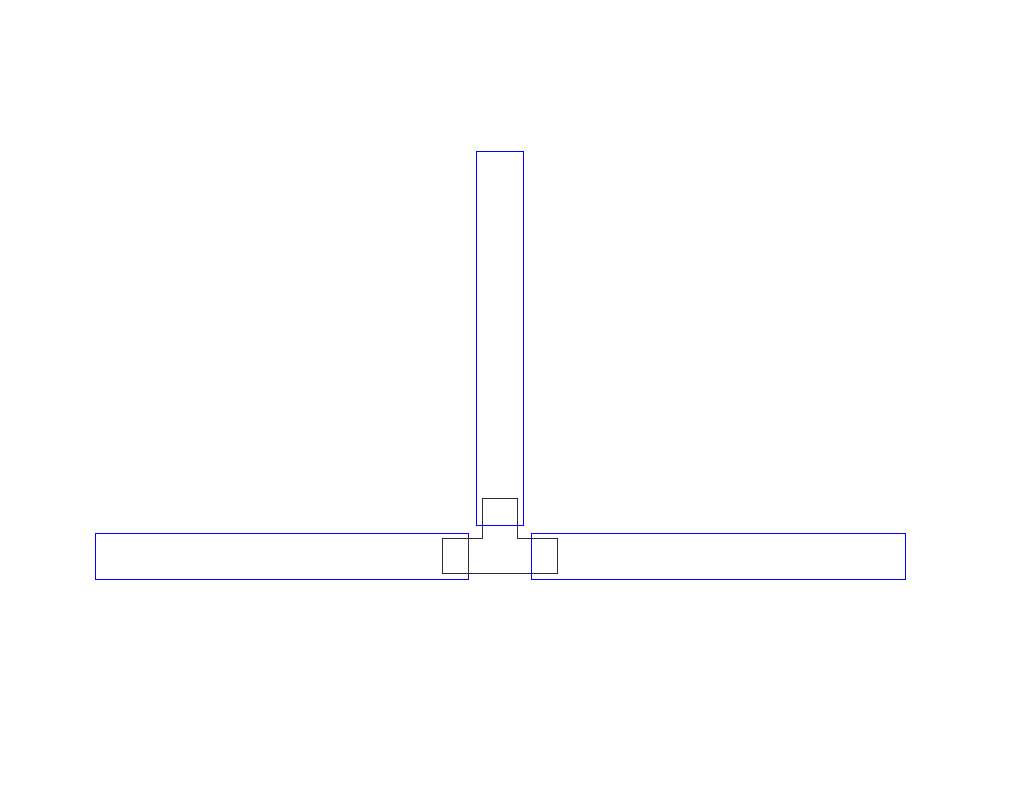
\includegraphics[width=\textwidth]{capturas/CAPTURA-AGUA-09-TE20.png}\\[0.15cm]
            \footnotesize \texttt{Te Ø20}
        \end{minipage}\hfill
        \begin{minipage}[t]{0.31\textwidth}
            \centering
            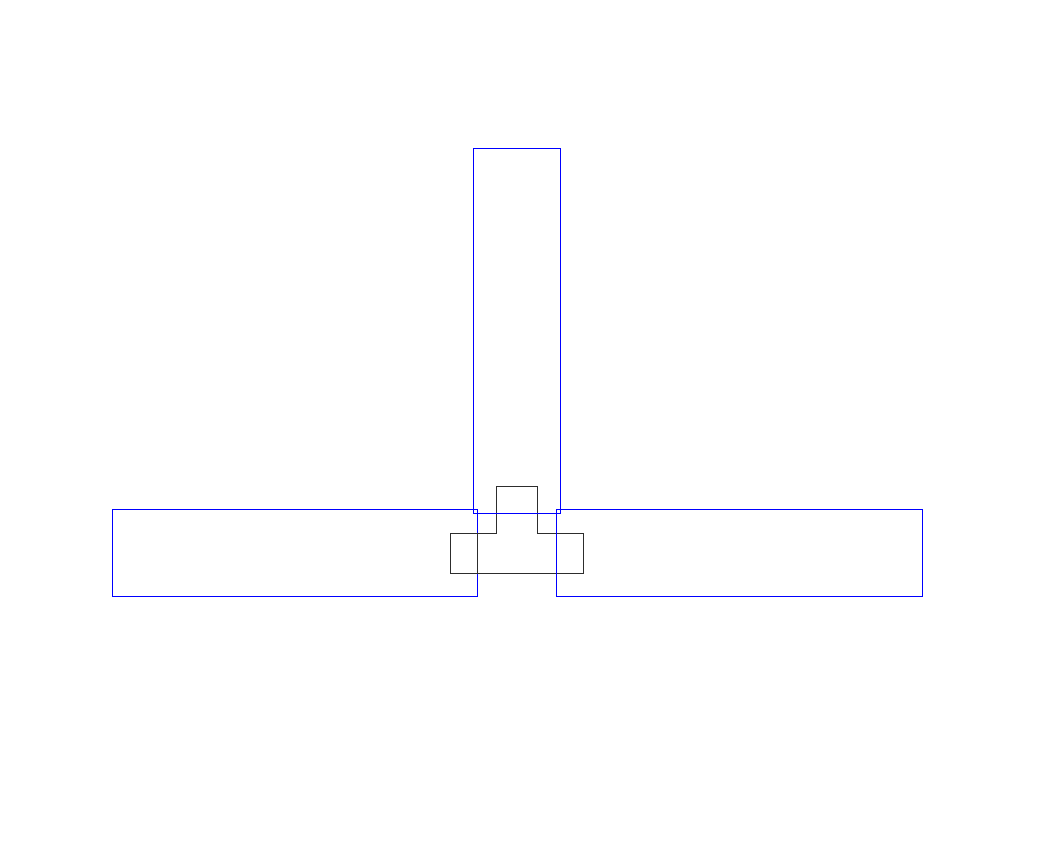
\includegraphics[width=\textwidth]{capturas/CAPTURA-AGUA-09-TE25.png}\\[0.15cm]
            \footnotesize \texttt{Te Ø25}
        \end{minipage}\hfill
        \begin{minipage}[t]{0.31\textwidth}
            \centering
            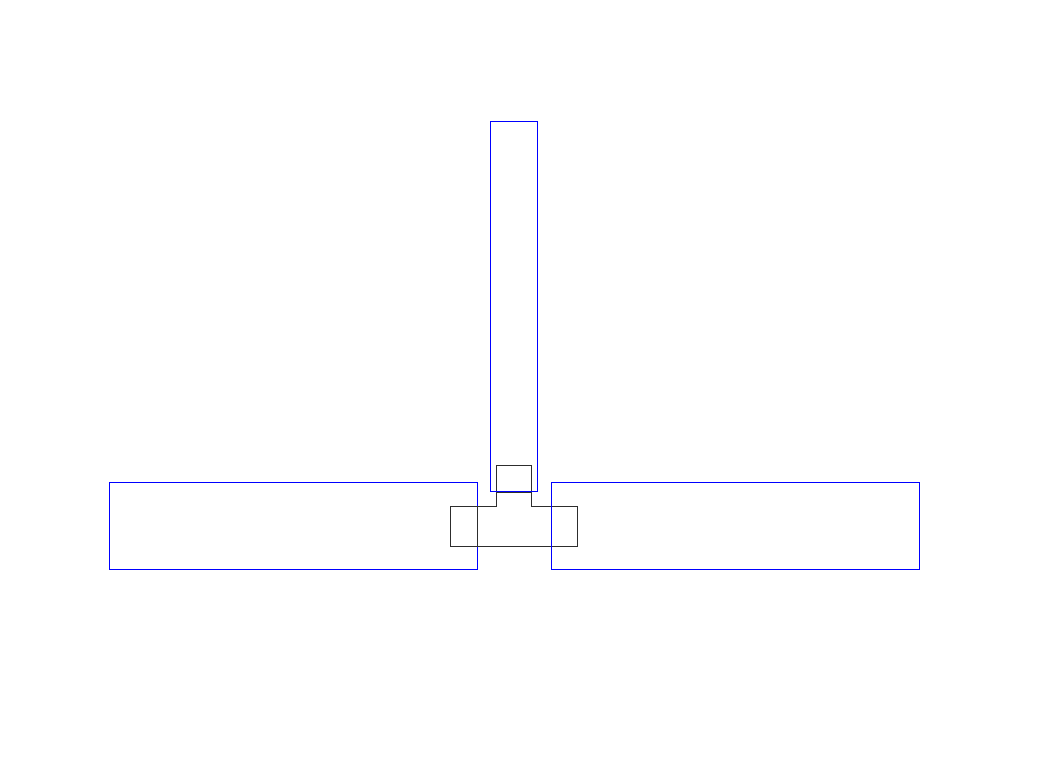
\includegraphics[width=\textwidth]{capturas/CAPTURA-AGUA-09-TE252025.png}\\[0.15cm]
            \footnotesize \texttt{Te Ø25-20-25}
        \end{minipage}\\[0.25cm]
        \hfill
        \begin{minipage}[t]{0.31\textwidth}
            \centering
            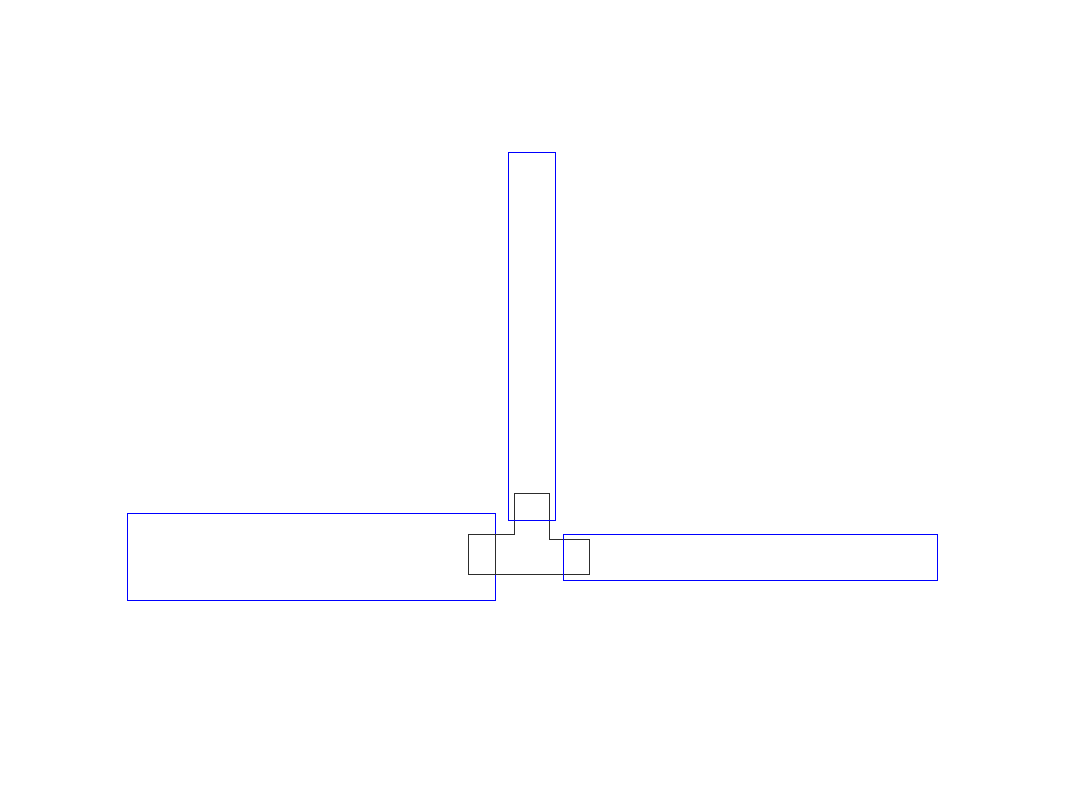
\includegraphics[width=\textwidth]{capturas/CAPTURA-AGUA-09-TE252020.png}\\[0.15cm]
            \footnotesize \texttt{Te Ø25-20-20}
        \end{minipage}\hfill
        \begin{minipage}[t]{0.31\textwidth}
            \centering
            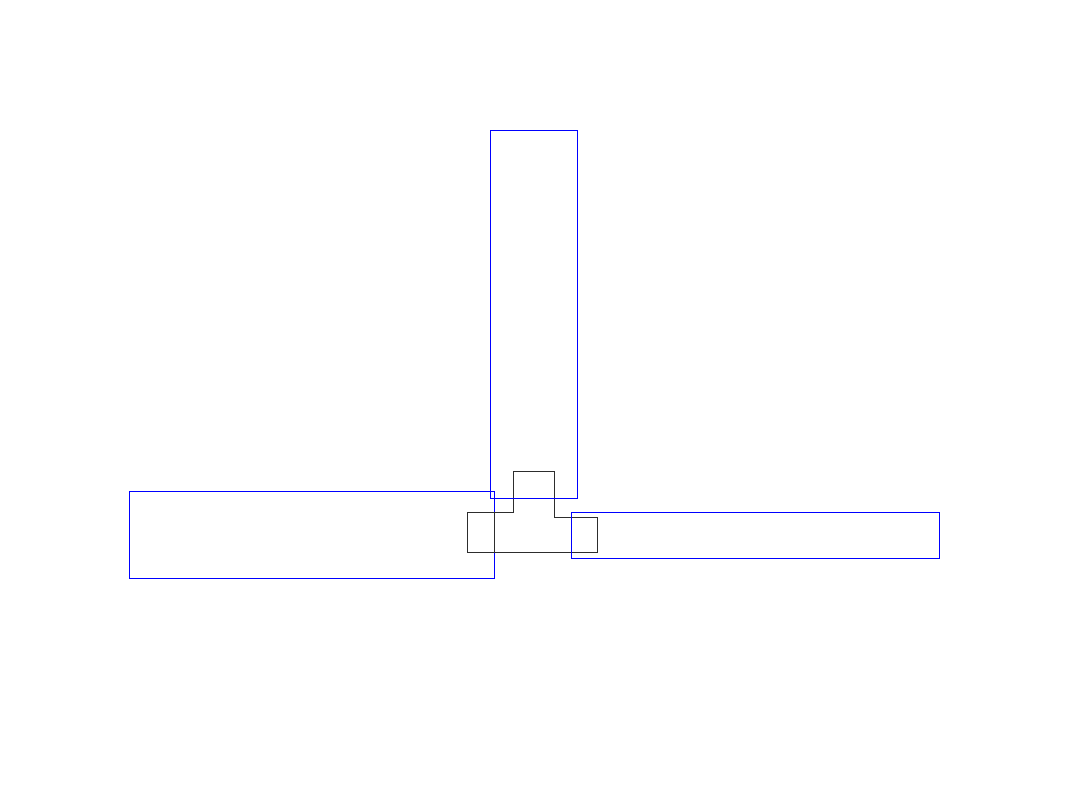
\includegraphics[width=\textwidth]{capturas/CAPTURA-AGUA-09-TE252520.png}\\[0.15cm]
            \footnotesize \texttt{Te Ø25-25-20}
        \end{minipage}
        \hfill
        \caption{Ejemplo comparativo de los distintos tipos de \texttt{Te} utilizados en Agua}
    \end{figure}
}{
    \placeholderimage{capturas/CAPTURA-AGUA-09-TE20.png / capturas/CAPTURA-AGUA-09-TE25.png / capturas/CAPTURA-AGUA-09-TE252025.png / capturas/CAPTURA-AGUA-09-TE252020.png / capturas/CAPTURA-AGUA-09-TE252520.png}{Ejemplo comparativo de los distintos tipos de \texttt{Te} utilizados en Agua}
}

\subsubsection{Qué ocurre si no existe una Te compatible}

Si la combinación de diámetros de entrada, salida y rama no tiene una \texttt{Te} disponible, la herramienta muestra un aviso indicando que no existe una \texttt{TE} para la combinación de diámetros seleccionada y pide modificar los diámetros de los segmentos para que coincidan con un tipo disponible.

\manualimage{capturas/CAPTURA-AGUA-10.png}{Aviso mostrado cuando no existe una Te para la combinación de diámetros seleccionada}

\subsection{Longitudes mínimas y máximas de tubo en Agua}

Además del sistema, la distribución y el diámetro, en Agua también hay condiciones de longitud que el usuario debe conocer.

\subsubsection{Longitud mínima}

La longitud mínima de tramo en la configuración actual es \texttt{350 mm}.

Si el usuario dibuja un segmento más corto:

\begin{itemize}
\item la herramienta muestra el tipo de instalación;
\item indica la longitud mínima requerida;
\item indica la longitud real del tramo dibujado;
\item y pregunta si se desea ignorar la restricción o cancelar para recolocar el punto.
\end{itemize}

Esto permite decidir en el momento si se mantiene ese tramo corto o si se corrige antes de seguir dibujando.

\manualimage{capturas/CAPTURA-AGUA-11.png}{Aviso de longitud mínima no cumplida al dibujar un tramo demasiado corto}

\subsubsection{Longitud máxima}

La longitud máxima de referencia en Agua es \texttt{5,00 m}.

Si un tramo supera esa longitud, la herramienta no muestra un aviso bloqueante, sino que divide automáticamente ese tramo en subtramos más cortos para poder resolver la instalación dentro del límite permitido.

Por eso, cuando se trabaja con recorridos largos, conviene revisar el resultado para comprobar dónde se han producido los cortes y cómo han quedado las uniones generadas.

\manualimage{capturas/CAPTURA-AGUA-12.png}{Ejemplo de tramo largo dividido automáticamente al superar la longitud máxima}

\subsection{Layers y atributo padre en Agua}

En Agua hay dos temas que conviene entender juntos:

\begin{itemize}
\item los \texttt{layers} de la instalación;
\item el valor que se aplica como \texttt{atributo padre};
\end{itemize}

\subsubsection{Layers propios de Agua}

En la configuración actual, Agua trabaja con una base de layers como:

\begin{itemize}
\item \texttt{AIGUA}
\item \texttt{AIGUA CARA X}
\item \texttt{AIGUA CARA Y}
\item \texttt{IS CON AIGUA FAB}
\item \texttt{IS CON AIGUA OBR}
\end{itemize}

Además, la instalación parte de un layer por defecto para la geometría principal y de un layer específico para la polilínea de eje cuando esta se genera como apoyo.

Por eso, aunque el usuario vea solo un desplegable de layers en la paleta, detrás hay una lógica propia de Agua que conviene respetar.

\manualimage{capturas/CAPTURA-AGUA-17.png}{Desplegable de layers de Agua mostrando las opciones disponibles en paleta}

\subsubsection{Qué debe entender el usuario sobre los layers en Agua}

Si el usuario no aplica un layer manualmente, la instalación utiliza su configuración por defecto.

Si el usuario selecciona elementos y usa \texttt{Aplicar layer}, esa asignación queda guardada para esos elementos y se utiliza al crear el resultado final.

Esto es especialmente importante en Agua cuando:

\begin{itemize}
\item se quiere distinguir fabricación y obra;
\item se necesita separar \texttt{Cara X} y \texttt{Cara Y};
\item o se quiere corregir la clasificación de un tramo o accesorio antes de finalizar.
\end{itemize}

En general, después de cambiar distribución, geometría o selección de elementos, conviene revisar también los layers.

\subsubsection{Casos en los que conviene revisar el layer final}

En Agua hay piezas, sobre todo en algunos casos \texttt{TD}, en las que la geometría puede resolverse con varias partes y no siempre interesa forzar todas ellas con el mismo criterio visual.

Por eso, si después de aplicar un layer el usuario ve una pieza que no responde exactamente como esperaba, conviene revisar el resultado final en pantalla en lugar de asumir que se trata de un error.

La regla práctica para el manual es esta:

\begin{itemize}
\item el layer aplicado desde paleta manda en el flujo habitual;
\item pero algunas piezas técnicas pueden conservar parte de su lógica propia de modelo.
\end{itemize}

\manualimage{capturas/CAPTURA-05.png}{Ejemplo de layer aplicado en Agua sobre tramos o accesorios seleccionados}

\subsubsection{Qué es el atributo padre en Agua}

En Agua, el \texttt{Valor atributo} que el usuario aplica desde la paleta no es solo una etiqueta descriptiva.

Ese valor se utiliza como \texttt{atributo padre}, que sirve para:

\begin{itemize}
\item identificar elementos que pertenecen a una misma referencia;
\item organizar la instalación;
\item y validar que la información esté completa antes de finalizar.
\end{itemize}

En Agua, la lógica es esta:

\begin{itemize}
\item en \texttt{TD}, el valor aplicado se utiliza como \texttt{pmp\_pare};
\item en \texttt{IS}, ese mismo valor se utiliza como \texttt{pmp\_pare} y también como \texttt{6\_CC\_IS}.
\end{itemize}

Es decir, el usuario escribe un único valor, pero la instalación lo reutiliza según la distribución activa.

\subsubsection{Cómo aplica el usuario el atributo padre}
\label{sec:agua-aplicar-atributo-padre}

El flujo práctico es:

\begin{enumerate}
\item seleccionar el tramo o los elementos que deban compartir referencia;
\item escribir el valor en el campo \texttt{Valor atributo};
\item pulsar \texttt{Aplicar atributo}.
\end{enumerate}

Cuando se hace esto, la herramienta confirma que los atributos han sido aplicados y guarda esa información para la creación final.

Si el usuario no asigna layer o atributo padre a ciertos elementos, antes de finalizar puede aparecer un aviso indicando que hay elementos sin configuración completa.

\manualimage{capturas/CAPTURA-AGUA-19.png}{Aplicación de Valor atributo en Agua y aviso de elementos sin layer o sin atributo padre}

\subsection{Elementos definidos propios de Agua}

Además del trazado automático, Agua permite insertar elementos definidos propios del sistema.

En la configuración actual, Agua trabaja con elementos definidos como:

\begin{itemize}
\item Colze Base;
\item Clau de Pas;
\item Taps;
\item T sortida.
\end{itemize}

Estos elementos se utilizan para completar la instalación con piezas concretas del sistema una vez que el recorrido principal ya está claro.

Además, algunos de estos elementos pueden mostrar un aviso si se intentan colocar en una distribución no admitida, especialmente en \texttt{IS}.

\manualimage{capturas/CAPTURA-AGUA-13.png}{Paleta de Elementos Definidos en Agua con los tipos disponibles}

\subsubsection{Tipo de punto en Elementos Definidos}

Además de elegir el elemento, en Agua es importante revisar el campo \texttt{Tipo de punto}, porque no todos los elementos pueden colocarse en cualquier posición de la instalación.

En la configuración actual, la relación es esta:

\begin{itemize}
\item \texttt{Colze base}: \texttt{Inicio} o \texttt{Final}.
\item \texttt{Taps}: \texttt{Inicio} o \texttt{Final}.
\item \texttt{T sortida}: \texttt{Intermedio ordenado} o \texttt{Intermedio libre}.
\item \texttt{Clau de Pas}: \texttt{Intermedio ordenado} o \texttt{Intermedio libre}.
\end{itemize}

\manualdoubleimagelabeled{capturas/CAPTURA-AGUA-13B1.png}{\texttt{T sortida}: \texttt{Intermedio ordenado} o \texttt{Intermedio libre}}{capturas/CAPTURA-AGUA-13B2.png}{\texttt{Colze base}: \texttt{Inicio} o \texttt{Final}}{Campo Tipo de punto en Elementos Definidos mostrando las opciones según el elemento seleccionado}

\subsubsection{Qué significa cada tipo de punto}

\begin{itemize}
\item \texttt{Inicio}: el elemento se coloca en el arranque de la polilínea o del recorrido correspondiente.
\item \texttt{Final}: el elemento se coloca en el extremo final del recorrido.
\item \texttt{Intermedio ordenado}: el elemento se coloca en una posición intermedia asociada al orden del recorrido.
\item \texttt{Intermedio libre}: el elemento se coloca en un punto intermedio elegido libremente por el usuario.
\end{itemize}

En otras palabras, \texttt{Inicio} y \texttt{Final} se usan para piezas que deben rematar o arrancar el recorrido, mientras que los tipos \texttt{Intermedio} se usan para piezas que deben quedar dentro del desarrollo de la instalación.

\subsubsection{Qué debe tener en cuenta el usuario}

\begin{itemize}
\item Si el elemento es de \texttt{Inicio/Final}, no debe intentarse como punto intermedio.
\item Si el elemento es intermedio, no debe intentarse como arranque o remate del recorrido.
\item Cuando la combinación no es válida, la herramienta avisa y no permite continuar con esa colocación.
\end{itemize}

Esto es especialmente importante en Agua porque el tipo de punto forma parte de la lógica de colocación del elemento, no es solo una etiqueta descriptiva.

\subsection{Soportes en Agua}

Además de las reglas comunes de soportes, en Agua hay particularidades de clasificación y de geometría que conviene revisar.

\subsubsection{Qué hace especial a los soportes de Agua}

En Agua no basta con fijarse en la forma del soporte. También hay que comprobar cómo queda asociado dentro de la instalación.

Esto es importante porque algunos soportes comparten familia geométrica con otras instalaciones. El caso más claro es \texttt{Omega}, ya que Agua y Saneamiento pueden trabajar con la misma base de soporte tipo \texttt{Varifix}.

Por eso, antes de insertar, conviene revisar que el campo \texttt{Subtipo instalación} quede realmente asociado a \texttt{Agua}. Si aparece otro subtipo, el soporte puede quedar clasificado como perteneciente a otra instalación aunque visualmente se parezca.

La confirmación previa a la inserción es un buen momento para comprobar \texttt{Tipo}, \texttt{Subtipo instalación}, \texttt{Superficie}, \texttt{Cota A}, \texttt{Cota B} y \texttt{Ángulo de inclinación} antes de continuar.

\manualimagesized{capturas/CAPTURA-14B.png}{Soporte de Agua con Subtipo instalación Agua visible en la paleta y en la confirmación previa a insertar}{0.60\textwidth}{0.55\textheight}

\subsubsection{Tipos de soporte más representativos en Agua}

En la configuración actual, los casos más representativos en Agua son:

\begin{itemize}
\item \texttt{Omega}, cuando se trabaja con la lógica de soporte \texttt{Varifix}.
\item \texttt{Zeta}, cuando se necesita un soporte lineal o un soporte con desarrollo vertical.
\item \texttt{Cinta}, cuando se resuelve el soporte mediante cinta.
\end{itemize}

La diferencia en Agua no depende solo de la forma. También depende de cómo quede clasificado el soporte dentro de la instalación.

\subsubsection{Cotas que cambian el resultado en Agua}

En Agua, las cotas no son un detalle menor, porque cambian directamente el tipo de resultado que se obtiene:

\begin{itemize}
\item en \texttt{Omega} asociado a Agua, \texttt{Cota A} y \texttt{Cota B} deben ser mayores que \texttt{0};
\item en \texttt{Zeta}, \texttt{Cota B} debe ser mayor que \texttt{0};
\item en \texttt{Zeta}, si \texttt{Cota A = 0 mm}, el soporte se resuelve como variante lineal \texttt{0 mm};
\item en \texttt{Zeta}, si \texttt{Cota A} es mayor que \texttt{0 mm}, el soporte pasa a una variante con desarrollo vertical;
\item en \texttt{Cinta}, la medida decisiva es \texttt{Cota B}, que también debe estar informada.
\end{itemize}

Esto conviene revisarlo siempre en previsualización, porque un mismo tipo de soporte puede dar un resultado muy distinto solo por cambiar las cotas.

\manualimage{capturas/CAPTURA-AGUA-15.png}{Comparación en Agua entre un soporte Zeta con Cota A igual a 0 mm y otro con Cota A mayor que 0 mm}

\subsubsection{Layers e identificación de soporte en Agua}

Cuando el soporte queda correctamente asociado a Agua, la clasificación habitual de salida es:

\begin{itemize}
\item layer \texttt{IS\_SUPORTS\_AIGUA};
\item o \texttt{IS\_SUPORTS\_AGUA}, si el proyecto usa esa nomenclatura;
\item denominación de soporte \texttt{SUPORT AIGUA}.
\end{itemize}

En cambio, el \texttt{Zeta 0 mm} mantiene su condición de soporte lineal y conserva la lógica de layer lineal general, en lugar de pasar al layer específico de Agua.

Esto es importante porque permite distinguir entre:

\begin{itemize}
\item soportes de Agua ya clasificados como parte de esa instalación;
\item y soportes lineales genéricos que no deben interpretarse igual.
\end{itemize}

\manualimagesized{capturas/CAPTURA-AGUA-16.png}{Propiedades finales de un soporte de Agua mostrando su layer e identificación}{0.50\textwidth}{0.60\textheight}

\subsubsection{Atributos de soporte en Agua}

En Agua, el \texttt{Atributo de soporte} no solo sirve para etiquetar visualmente el soporte. También ayuda a dejarlo correctamente identificado dentro de la instalación.

Si el flujo del proyecto utiliza organización por atributo padre, conviene revisar este valor antes de finalizar, porque puede influir en cómo se organiza el soporte dentro de la instalación.

Por eso, cuando los soportes formen parte de una misma sectorización o deban seguir la misma lógica que la instalación principal, es recomendable aplicar ese atributo antes de cerrar el trabajo.

\subsubsection{Qué conviene revisar antes de acumular o finalizar soportes en Agua}

\begin{itemize}
\item que \texttt{Subtipo instalación} sea realmente \texttt{Agua};
\item que un \texttt{Omega} no se haya quedado clasificado como otra instalación que use la misma familia de soporte;
\item que \texttt{Cota A} y \texttt{Cota B} correspondan al tipo de soporte elegido;
\item que un \texttt{Zeta 0 mm} no se haya usado por error cuando se necesitaba un soporte con desarrollo vertical;
\item que el layer y la identificación final del soporte sean los esperados;
\item y que el \texttt{Atributo de soporte} esté informado si el proyecto necesita clasificación por atributo.
\end{itemize}

\subsection{Puntos a revisar con especial atención en Agua}

Antes de finalizar una instalación de Agua conviene revisar especialmente:

\begin{itemize}
\item que el sistema seleccionado sea realmente \texttt{Polietilè}, \texttt{Multicapa} o \texttt{Armaflex}, según el caso;
\item que la distribución sea la correcta y, si procede, que \texttt{Cara (EN)} también esté bien definida;
\item que después de un cambio de diámetro se hayan regenerado correctamente codos, manguitos reductores y Tes, especialmente si la reducción aparece justo después de un codo;
\item que los giros del recorrido respondan a la lógica de \texttt{90 grados};
\item que los avisos de longitud mínima se hayan resuelto conscientemente;
\item que los layers de Agua se correspondan con el criterio de trabajo que se necesita en ese plano;
\item que el atributo padre se haya aplicado realmente a los elementos que deben compartir referencia;
\item que los soportes de Agua hayan quedado asociados al subtipo correcto, con sus cotas y layers bien resueltos;
\item y que los recorridos largos no hayan generado divisiones automáticas en puntos no deseados.
\end{itemize}

\section{Instalación de Saneamiento}

En esta unidad solo se recogen las particularidades de Saneamiento. El uso general de la herramienta ya se ha explicado en los apartados anteriores, por lo que aquí se detallan únicamente las reglas, avisos y casos propios de esta instalación.

\subsection{Sistemas disponibles en Saneamiento}

En la instalación de Saneamiento, el usuario puede trabajar con estos sistemas:

\begin{itemize}
\item Pluvial;
\item Fecal.
\end{itemize}

La diferencia práctica entre ambos no está solo en el nombre del sistema, sino también en el catálogo de diámetros que puede utilizarse.

En la configuración actual:

\begin{itemize}
\item \texttt{Pluvial} trabaja con una configuración más limitada de diámetro;
\item \texttt{Fecal} permite más opciones.
\end{itemize}

Cuando el usuario cambia de sistema, la herramienta adapta automáticamente el comportamiento del trazado y los elementos que se colocan sobre él.

\manualimage{capturas/CAPTURA-SANEAMIENTO-01.png}{Paleta de Saneamiento con los sistemas Pluvial y Fecal visibles}

\subsection{Distribuciones en Saneamiento}

En la configuración actual, Saneamiento no utiliza la distribución como un parámetro práctico de trabajo para el usuario.

Por eso, a diferencia de Agua, aquí no hace falta documentar combinaciones especiales de distribución. Para el uso diario, lo importante es revisar el sistema activo, el diámetro y el sentido del trazado.

\subsection{Diámetros y cambios de diámetro en Saneamiento}

En Saneamiento, el diámetro disponible depende del sistema seleccionado.

\subsubsection{Diámetros por sistema}

En la configuración actual:

\begin{itemize}
\item \texttt{Pluvial}: \texttt{110 mm};
\item \texttt{Fecal}: \texttt{25 mm}, \texttt{40 mm} y \texttt{110 mm}.
\end{itemize}

Esto significa que, antes de dibujar o de modificar un tramo, conviene comprobar primero qué sistema está activo.

\manualimage{capturas/CAPTURA-SANEAMIENTO-02.png}{Selector de diámetro en Saneamiento con las opciones visibles para Fecal}

\subsubsection{Qué ocurre al cambiar el diámetro de un tramo}

Cuando el usuario modifica el diámetro de un tramo:

\begin{itemize}
\item se actualiza ese tramo;
\item se recalculan automáticamente las uniones cercanas;
\item y se regeneran los accesorios afectados en esa zona.
\end{itemize}

Por eso, después de un cambio de diámetro conviene revisar el resultado local, no solo el tramo modificado.

\manualimage{capturas/CAPTURA-SANEAMIENTO-03.png}{Acción Modificar diámetro aplicada sobre un tramo de Saneamiento}

\subsubsection{Qué ocurre si hay dos tramos consecutivos en línea recta con distinto diámetro}

Si dos tramos consecutivos siguen en línea recta pero cambian de diámetro, la herramienta coloca automáticamente una unión de transición o reducción.

Este es el caso habitual para resolver una transición recta entre dos diámetros distintos.

\manualimage{capturas/CAPTURA-SANEAMIENTO-04.png}{Transición automática de diámetro entre dos tramos rectos consecutivos}

\subsubsection{Qué ocurre si el cambio de diámetro afecta a un codo}

Si el cambio de diámetro afecta a un giro, la herramienta recalcula el codo y reajusta la unión de la zona afectada.

Cuando antes y después del giro aparecen diámetros distintos, conviene revisar en pantalla cómo ha quedado resuelto el encuentro, porque el resultado final depende de la combinación entre el giro y la transición de diámetro.

\subsubsection{Qué ocurre si el cambio de diámetro afecta a una bifurcación}

Si el cambio de diámetro afecta a una bifurcación, la herramienta intenta colocar la pieza compatible con la combinación detectada.

Si no existe una combinación válida, aparece un aviso como este:

\texttt{No existe una TE para la combinación de diámetros seleccionada.}

\texttt{Combinación detectada: ...}

\texttt{Modifique los diámetros de los segmentos para que coincidan con los tipos de TE disponibles.}

En ese caso, el usuario debe revisar los diámetros de la entrada, la salida y la rama hasta encajar con una combinación disponible.

\manualimage{capturas/CAPTURA-SANEAMIENTO-07.png}{Aviso mostrado cuando no existe una bifurcación compatible en Saneamiento}

\subsection{Accesorios automáticos en Saneamiento}

En Saneamiento, los accesorios automáticos dependen de la geometría del recorrido, del diámetro de los tramos y también del sentido del trazado.

\subsubsection{Codos}

En Saneamiento la resolución automática de giros puede hacerse con:

\begin{itemize}
\item \texttt{codos de 45 grados};
\item \texttt{codos de 90 grados}.
\end{itemize}

Esto la diferencia claramente de Agua, donde el comportamiento habitual documentado es el codo de \texttt{90 grados}.

\manualimage{capturas/CAPTURA-SANEAMIENTO-05.png}{Ejemplo comparativo de un codo de 45 grados y un codo de 90 grados en Saneamiento}

\subsubsection{Uniones y reducciones}

Cuando dos tramos consecutivos están alineados:

\begin{itemize}
\item si mantienen el mismo diámetro, la herramienta coloca una unión;
\item si cambian de diámetro, la unión se resuelve mediante una transición o reducción.
\end{itemize}

Este comportamiento debe revisarse especialmente después de modificar el diámetro de un tramo ya dibujado.

\subsubsection{Bifurcaciones}

Cuando en un mismo punto confluyen tres direcciones, la instalación intenta resolver el encuentro con la bifurcación compatible.

En Saneamiento se trabaja con bifurcaciones tipo \texttt{Y} y con algunas bifurcaciones de transición en casos concretos.

\manualimage{capturas/CAPTURA-SANEAMIENTO-06.png}{Ejemplo de bifurcación válida en Saneamiento}

\subsubsection{Qué ocurre si no existe una bifurcación compatible}

No todas las combinaciones de diámetro están disponibles en bifurcación.

Cuando no existe una pieza compatible, la herramienta muestra el aviso correspondiente y el usuario debe corregir los diámetros hasta adaptarlos a una combinación admitida.

\subsection{Reglas geométricas y validaciones en Saneamiento}

Además del sistema y del diámetro, en Saneamiento hay reglas geométricas que conviene tener presentes.

\subsubsection{Longitud mínima}

La longitud mínima de tramo indicada para Saneamiento es \texttt{350 mm}.

Si el usuario dibuja un tramo por debajo de ese valor, el resultado puede no resolverse correctamente.

\pendingtag\ El mensaje exacto de esa validación debe confirmarse en Allplan antes del cierre definitivo del manual.

\subsubsection{Longitud máxima}

\pendingtag\ La longitud máxima de tramo en Saneamiento debe confirmarse en Allplan.

Por eso, antes de cerrar la versión final de esta unidad conviene validar en entorno real:

\begin{itemize}
\item si existe un límite máximo;
\item qué ocurre cuando se supera;
\item y si aparece o no un aviso específico.
\end{itemize}

\subsubsection{Ajustes automáticos y sentido del trazado}

En Saneamiento, la herramienta recorta automáticamente algunos extremos de tramo para poder encajar los accesorios.

Además, el sentido del trazado influye en el resultado de determinadas piezas. Por eso, el usuario no debe fijarse solo en la geometría, sino también en la dirección en la que se ha construido el recorrido.

Esto es importante porque existe la acción \texttt{Invertir caval}, que permite cambiar el sentido de la instalación cuando el resultado geométrico no es el esperado.

\manualimage{capturas/CAPTURA-SANEAMIENTO-13.png}{Botón Invertir caval con mensaje de confirmación en Saneamiento}

\subsection{Layers y atributos en Saneamiento}

En Saneamiento conviene revisar tres cosas:

\begin{itemize}
\item los layers aplicados;
\item los atributos aplicados sobre la selección;
\item y que el resultado final quede clasificado según el criterio del plano.
\end{itemize}

\subsubsection{Layers que conviene revisar}

En Saneamiento conviene revisar especialmente estos layers:

\begin{itemize}
\item \texttt{IS CON SANE FAB};
\item \texttt{IS CON SANE OBR}.
\end{itemize}

\pendingtag\ También se mencionan otros layers de proyecto que conviene validar en Allplan antes de cerrar definitivamente esta unidad del manual.

\manualimage{capturas/CAPTURA-SANEAMIENTO-11.png}{Aplicación de layer sobre tramos o accesorios de Saneamiento}

\subsubsection{Atributos que conviene revisar}

El funcionamiento para aplicar atributos sobre elementos seleccionados es el mismo que en Agua.

Para ver el flujo paso a paso y la captura de ejemplo, consultar el apartado~\ref{sec:agua-aplicar-atributo-padre}.

En Saneamiento conviene revisar además los atributos de soporte aplicados desde la página específica de soportes.

\pendingtag\ Los atributos padre o campos críticos de Saneamiento todavía deben confirmarse.

\subsection{Elementos definidos propios de Saneamiento}

En la paleta de Saneamiento aparece, como elemento definido principal:

\begin{itemize}
\item \texttt{Caixa Connexions 200}.
\end{itemize}

Su función es insertar un elemento de conexión o registro sobre un punto de la instalación.

Suele ser útil:

\begin{itemize}
\item en puntos de inicio;
\item en puntos finales;
\item y en puntos intermedios donde se necesite resolver una conexión o un registro.
\end{itemize}

\manualimage{capturas/CAPTURA-SANEAMIENTO-08.png}{Uso de Caixa Connexions 200 en Saneamiento}

\subsubsection{Tipos de punto admitidos}

En la paleta, \texttt{Caixa Connexions 200} admite:

\begin{itemize}
\item \texttt{Inicio};
\item \texttt{Final};
\item \texttt{Intermedio ordenado};
\item \texttt{Intermedio libre}.
\end{itemize}

En paleta, la opción intermedia puede aparecer como \texttt{Intermedio o libre}.

\pendingtag\ El mensaje exacto mostrado cuando se intenta usar un tipo de punto no válido todavía debe confirmarse.

\subsection{Soportes en Saneamiento}

Saneamiento dispone también de una página específica de soportes.

En la paleta de soportes:

\begin{itemize}
\item el tipo \texttt{Zeta} aparece como valor visible por defecto;
\item las superficies habituales son \texttt{Liso} y \texttt{Perforado};
\item y el flujo de trabajo incluye inserción, creación y edición desde la misma paleta.
\end{itemize}

También conviene revisar:

\begin{itemize}
\item \texttt{Cota A};
\item \texttt{Cota B};
\item y \texttt{Ángulo de inclinación}.
\end{itemize}

\pendingtag\ El listado completo de tipos de soporte de Saneamiento todavía debe confirmarse.

\manualimage{capturas/CAPTURA-SANEAMIENTO-10.png}{Página de soportes de Saneamiento con inserción y edición}

\subsection{Mensajes y avisos propios de Saneamiento}

En Saneamiento pueden aparecer estos avisos relevantes:

\begin{itemize}
\item \texttt{No hay instalación guardada para invertir.}

Aparece al intentar invertir una instalación sin trazado guardado.

\item \texttt{Instalación invertida: ahora va de final a inicio.}

Aparece cuando la inversión se realiza correctamente.

\item \texttt{No se pudo invertir la instalación: ...}

Aparece cuando la inversión falla y conviene revisar el trazado.

\item \texttt{No existe una TE para la combinación de diámetros seleccionada...}

Aparece cuando no existe una bifurcación compatible con los diámetros detectados.

\item \texttt{caval sin sentido sera creado}

Aparece en casos concretos relacionados con la orientación de la bifurcación.
\end{itemize}

\pendingtag\ Conviene validar estos mensajes en Allplan antes del cierre definitivo del manual, especialmente si alguno de ellos se ha abreviado en la información inicial.

\subsection{Puntos a revisar con especial atención en Saneamiento}

Antes de finalizar una instalación de Saneamiento conviene revisar especialmente:

\begin{itemize}
\item que el sistema activo sea realmente \texttt{Pluvial} o \texttt{Fecal};
\item que el diámetro elegido sea compatible con ese sistema;
\item que los cambios de diámetro hayan regenerado correctamente uniones, reducciones, codos y bifurcaciones;
\item que una bifurcación no haya quedado en una combinación no válida;
\item que los giros se estén resolviendo con el ángulo esperado, especialmente en casos de \texttt{45 grados} y \texttt{90 grados};
\item que los avisos de longitud mínima se hayan resuelto conscientemente;
\item que el sentido del trazado sea el correcto antes de usar \texttt{Invertir caval};
\item que los layers y atributos aplicados respondan al criterio del plano;
\item que \texttt{Caixa Connexions 200} esté colocada con el tipo de punto adecuado;
\item y que los soportes se hayan revisado con sus cotas, superficie y tipo correctos.
\end{itemize}

\section{Instalación de Ventilación}

En esta unidad solo se recogen las particularidades de Ventilación. El uso general de la herramienta ya se ha explicado en los apartados anteriores, por lo que aquí se detallan únicamente las reglas, avisos y casos propios de esta instalación.

\subsection{Descripción general de Ventilación}

Ventilación sirve para dibujar y editar redes de conductos dentro de Allplan.

El usuario define un recorrido y la herramienta genera los tramos y accesorios correspondientes según el sistema elegido.

Lo que diferencia a Ventilación de otras instalaciones es la combinación de tipos de conducto, diámetros, ángulos permitidos y accesorios específicos como manguitos, difusores, reducciones, conexiones y codos.

\subsection{Sistemas disponibles en Ventilación}

En la configuración actual de Ventilación aparecen estos sistemas:

\begin{itemize}
\item \texttt{Conducto Impulsion};
\item \texttt{Conducto Extraccion};
\item \texttt{Conducto Aislado};
\item \texttt{Conducto Recuperador}.
\end{itemize}

Las diferencias principales entre ellos son estas:

\begin{itemize}
\item \texttt{Conducto Impulsion} y \texttt{Conducto Extraccion} comparten geometría base, pero usan color y artículo distintos.
\item \texttt{Conducto Aislado} trabaja con conducto dinámico y con reducción como conexión característica.
\item \texttt{Conducto Recuperador} trabaja con otra lógica de generación y solo admite giros de \texttt{90 grados}.
\end{itemize}

Cuando el usuario cambia de sistema, la herramienta adapta automáticamente el comportamiento del trazado, el diámetro base y los accesorios disponibles.

\manualimage{capturas/CAPTURA-VENTILACION-01.png}{Paleta de Ventilación con los cuatro sistemas visibles}

\subsection{Distribución en Ventilación}

En la paleta existe el campo \texttt{Tipo de Distribucion}, pero en la paleta actual de Ventilación no aparece una distribución funcional específica como sí ocurre en Agua.

Por eso, para esta instalación:

\begin{itemize}
\item \pendingtag\ debe validarse si este campo se usa realmente o si permanece sin aplicación práctica para el usuario.
\end{itemize}

\subsection{Diámetros y cambios de diámetro en Ventilación}

\subsubsection{Diámetros por sistema}

Los diámetros confirmados en la configuración actual son:

\begin{itemize}
\item \texttt{Conducto Impulsion}: \texttt{75 mm};
\item \texttt{Conducto Extraccion}: \texttt{75 mm};
\item \texttt{Conducto Aislado}: \texttt{150 mm} y \texttt{160 mm};
\item \texttt{Conducto Recuperador}: \texttt{160 mm}.
\end{itemize}

Esto significa que el diámetro disponible depende del sistema seleccionado.

\manualimage{capturas/CAPTURA-VENTILACION-02.png}{Selector de diámetro en Conducto Aislado mostrando 150 mm y 160 mm}

\subsubsection{Qué ocurre al modificar el diámetro}

El botón \texttt{Modificar diámetro} recalcula el tramo y las uniones afectadas.

Cuando el cambio de diámetro se produce entre dos tramos consecutivos en línea recta:

\begin{itemize}
\item en conductos compatibles, la herramienta genera automáticamente la transición o la unión correspondiente.
\end{itemize}

En los sistemas donde existen accesorios automáticos, conviene revisar en pantalla cómo se rehace la unión después del cambio.

\subsubsection{Caso particular de Conducto Aislado}

En \texttt{Conducto Aislado}, la conexión característica es la \texttt{reducción}.

Por eso, cuando el usuario trabaja con \texttt{150 mm} y \texttt{160 mm}, conviene revisar explícitamente la transición resultante.

\subsection{Accesorios automáticos en Ventilación}

Los accesorios automáticos dependen del sistema seleccionado.

En el uso actual, el comportamiento previsto es:

\begin{itemize}
\item \texttt{Conducto Impulsion} y \texttt{Conducto Extraccion}: \texttt{manguito} y \texttt{difusor};
\item \texttt{Conducto Aislado}: \texttt{reducción};
\item \texttt{Conducto Recuperador}: \texttt{conexion} y \texttt{codo 90}.
\end{itemize}

Los accesorios principales que conviene reconocer en Ventilación son:

\begin{itemize}
\item \texttt{Manguito};
\item \texttt{Difusor};
\item \texttt{Conexion};
\item \texttt{Codo 90}.
\end{itemize}

\subsubsection{Manguitos}

En los sistemas normales, el manguito no actúa solo como accesorio visual.

También ayuda a separar o resolver tramos del recorrido cuando la instalación necesita ordenar la continuidad del conducto.

\manualimage{capturas/CAPTURA-VENTILACION-03.png}{Ejemplo de Conducto Impulsion con manguito automático}

\subsubsection{Difusores}

En los sistemas que los usan, los difusores forman parte del comportamiento automático previsto por la instalación.

Conviene revisar su colocación final cuando el trazado cambia de dirección o de plano.

\manualimage{capturas/CAPTURA-VENTILACION-04.png}{Ejemplo de Conducto Extraccion con difusor}

\subsubsection{Recuperador con conexión y codo}

En \texttt{Conducto Recuperador}, el flujo de creación trabaja con un conjunto de piezas encadenadas:

\begin{itemize}
\item conducto;
\item conexión;
\item codo.
\end{itemize}

Esto lo diferencia claramente del resto de sistemas de Ventilación.

\manualimage{capturas/CAPTURA-VENTILACION-05.png}{Recuperador con conexión y codo 90}

\subsubsection{Limitaciones o incompatibilidades}

\texttt{Conducto Recuperador} no sigue la misma lógica de ángulos que el resto.

\begin{itemize}
\item \pendingtag\ debe validarse si aparecen avisos específicos cuando el usuario intenta forzar una combinación no compatible.
\end{itemize}

\subsection{Reglas geométricas y validaciones en Ventilación}

\subsubsection{Ángulos permitidos}

Los ángulos generales soportados en la instalación son:

\begin{itemize}
\item \texttt{45 grados};
\item \texttt{90 grados}.
\end{itemize}

Por sistema, la regla actual es esta:

\begin{itemize}
\item \texttt{Conducto Impulsion} y \texttt{Conducto Extraccion}: \texttt{45} y \texttt{90 grados};
\item \texttt{Conducto Aislado}: \texttt{45} y \texttt{90 grados};
\item \texttt{Conducto Recuperador}: solo \texttt{90 grados}.
\end{itemize}

\subsubsection{Longitud mínima}

La longitud mínima por sistema es:

\begin{itemize}
\item \texttt{Conducto Impulsion} y \texttt{Conducto Extraccion}: \texttt{300 mm};
\item \texttt{Conducto Aislado}: \texttt{300 mm};
\item \texttt{Conducto Recuperador}: \texttt{350 mm}.
\end{itemize}

Si el usuario dibuja un segmento más corto que la longitud mínima permitida, la herramienta muestra un aviso con:

\begin{itemize}
\item el tipo de instalación;
\item la longitud mínima requerida;
\item la longitud real del segmento trazado;
\item y la pregunta para decidir si se ignora la restricción o se cancela para recolocar el punto.
\end{itemize}

\manualdoubleimagelabeled
{capturas/CAPTURA-VENTILACION-06A.png}
{\texttt{Conducto Impulsion}}
{capturas/CAPTURA-VENTILACION-06B.png}
{\texttt{Conducto Extraccion}}
{Avisos de longitud mínima no cumplida en Conducto Impulsion y Conducto Extraccion}

\manualdoubleimagelabeled
{capturas/CAPTURA-VENTILACION-06C.png}
{\texttt{Conducto Aislado}}
{capturas/CAPTURA-VENTILACION-06D.png}
{\texttt{Conducto Recuperador}}
{Avisos de longitud mínima no cumplida en Conducto Aislado y Conducto Recuperador}

\subsection{Layers y atributos específicos de Ventilación}

\subsubsection{Layers base}

Los layers base que conviene revisar en Ventilación son:

\begin{itemize}
\item \texttt{IS\_CON\_VENT\_FAB};
\item \texttt{IS\_CON\_VENT\_FAB\_SOB1};
\item \texttt{IS\_CON\_VENT\_OBRA};
\item \texttt{IS\_CON\_VENT\_EIX};
\item \texttt{IS\_NOM\_CONDUCTE\_VENTILACIO}.
\end{itemize}

Esto cubre tanto los conductos como la capa de eje y la capa de etiqueta o nombre del conducto.

\manualimage{capturas/CAPTURA-VENTILACION-06.png}{Ejemplo de layer aplicado en Ventilación}

\subsubsection{Atributos que conviene revisar}

En Ventilación, los atributos sirven para clasificar el conducto y completar información como referencia, dimensiones, longitud, sección o tipo de sistema.

Para el usuario, lo importante es comprobar que los atributos necesarios del proyecto se han aplicado antes de finalizar la instalación.

Conviene revisar especialmente:

\begin{itemize}
\item que el atributo de referencia o clasificación esté informado cuando el proyecto lo requiera;
\item que el sistema elegido se corresponda con el uso real del conducto;
\item y que los elementos especiales, como recuperadores o difusores, no queden sin información necesaria.
\end{itemize}

\subsection{Elementos definidos en Ventilación}

En Ventilación hay que distinguir entre dos tipos de elementos:

\begin{itemize}
\item accesorios que la herramienta coloca automáticamente al generar el recorrido;
\item elementos que el usuario puede insertar manualmente desde la página \texttt{Elemento}.
\end{itemize}

Los accesorios propios de Ventilación que deben revisarse en el modelo son:

\begin{itemize}
\item \texttt{Manguito};
\item \texttt{Difusor};
\item \texttt{Conducto recuperador};
\item \texttt{Conexion};
\item \texttt{Codo 90}.
\end{itemize}

En la página \texttt{Elemento} puede aparecer actualmente:

\begin{itemize}
\item \texttt{Caixa Connexions 200}.
\end{itemize}

Por tanto, antes de cerrar esta unidad del manual, conviene validar en Allplan si \texttt{Caixa Connexions 200} es realmente el elemento que debe insertar el usuario en Ventilación o si la paleta debe mostrar otro elemento propio de esta instalación.

\pendingtag\ Validar qué elementos definidos ve el usuario en la paleta de Ventilación y cuáles se generan solo de forma automática.

\manualimage{capturas/CAPTURA-VENTILACION-10.png}{Página de Elemento mostrando el estado real en Ventilación}

\subsection{Soportes en Ventilación}

Ventilación dispone de página específica de soportes.

Los campos visibles en paleta son:

\begin{itemize}
\item \texttt{Tipo de soporte};
\item \texttt{Subtipo instalación};
\item \texttt{Superficie};
\item \texttt{Cota A};
\item \texttt{Cota B};
\item \texttt{Ángulo de inclinación};
\item modos de edición de soportes;
\item y \texttt{Atributo de soporte}.
\end{itemize}

En la paleta puede aparecer al menos un soporte \texttt{Omega}, con subtipo \texttt{Ventilacion} y superficie \texttt{Perforado}.

Las reglas prácticas de uso son estas:

\begin{itemize}
\item conviene definir tipo, superficie y cotas antes de insertar;
\item los soportes pueden acumularse y crearse después;
\item el modo \texttt{Edición Mover} permite recolocar soportes ya acumulados o seleccionados.
\end{itemize}

\pendingtag\ Debe confirmarse el listado completo de tipos de soporte realmente habilitados en Ventilación.

\manualimage{capturas/CAPTURA-VENTILACION-07.png}{Bloque de soportes con subtipo Ventilacion}

\subsection{Mensajes y avisos propios de Ventilación}

En esta instalación todavía deben confirmarse los avisos que verá realmente el usuario en Allplan.

Conviene validar en entorno real:

\begin{itemize}
\item el aviso por longitud mínima;
\item el aviso por selección o inserción inválida;
\item el aviso por combinación de geometría no soportada en recuperador;
\item y los mensajes de finalización si falta configuración de layers o atributos.
\end{itemize}

\subsection{Puntos a revisar con especial atención en Ventilación}

Antes de finalizar una instalación de Ventilación conviene revisar especialmente:

\begin{itemize}
\item que el sistema activo sea realmente \texttt{Conducto Impulsion}, \texttt{Conducto Extraccion}, \texttt{Conducto Aislado} o \texttt{Conducto Recuperador};
\item que el diámetro elegido sea compatible con ese sistema;
\item que en \texttt{Conducto Aislado} la transición entre \texttt{150 mm} y \texttt{160 mm} se haya resuelto correctamente;
\item que en \texttt{Conducto Recuperador} los giros respondan a la lógica de \texttt{90 grados};
\item que los layers aplicados correspondan al criterio del plano;
\item que los atributos de clasificación se hayan aplicado como se espera;
\item que la página de \texttt{Elemento} esté mostrando el elemento correcto para esta instalación;
\item y que los soportes se hayan revisado con subtipo, superficie, cotas y tipo correctos.
\end{itemize}

\section{Instalación de Electricidad}

En esta unidad solo se recogen las particularidades de Electricidad. El uso general de la herramienta ya se ha explicado en los apartados anteriores, por lo que aquí se detallan únicamente las reglas, avisos y casos propios de esta instalación.

\subsection{Descripción general de Electricidad}

Electricidad sirve para dibujar y editar recorridos eléctricos dentro de Allplan.

Está pensada para trabajar tanto con \texttt{Rejibands} como con conductos o corrugados asociados a distintos usos eléctricos.

Lo que diferencia a Electricidad de otras instalaciones es la variedad de recorridos disponibles, la separación entre corrugados eléctricos y telecomunicaciones, y la posibilidad de trabajar con variantes de distribución según el proyecto.

\subsection{Sistemas disponibles en Electricidad}

En la configuración actual de Electricidad aparecen estos sistemas:

\begin{itemize}
\item \texttt{Rejiband U 100mm};
\item \texttt{Rejiband U 200mm};
\item \texttt{Telecomunicaciones};
\item \texttt{Luz retorno / Paralelas};
\item \texttt{Alimentación horno};
\item \texttt{Alimentación luces / Cajetines};
\item \texttt{Cajetín a enchufe};
\item \texttt{Interruptores / Domótica}.
\end{itemize}

Las diferencias principales entre ellos son estas:

\begin{itemize}
\item \texttt{Rejiband U 100mm} y \texttt{Rejiband U 200mm} trabajan como soporte lineal principal con ancho diferente.
\item El resto trabajan como conductos o corrugados asociados a usos concretos de la instalación eléctrica.
\item Cada tipo define color, diámetro base, solape y lógica geométrica propia.
\end{itemize}

\manualimage{capturas/CAPTURA-ELECTRICIDAD-01.png}{Paleta de Electricidad con los sistemas disponibles visibles}

\subsection{Distribución y variantes en Electricidad}

En la paleta puede aparecer el campo \texttt{Tipo de Distribucion}.

Electricidad puede trabajar con una lógica base y con variantes de distribución como \texttt{TD}. Además, la paleta incluye el campo \texttt{Cara (EN)}, que puede usarse para definir la cara o criterio de colocación en determinados recorridos.

Para el usuario, la regla práctica es revisar estos campos antes de dibujar, especialmente si el proyecto diferencia entre recorridos base, recorridos \texttt{TD} o recorridos asociados a una cara concreta.

\pendingtag\ Debe validarse cómo selecciona realmente el usuario la variante \texttt{TD} o \texttt{EN} en Electricidad y qué efecto visible tiene en el recorrido.

\subsection{Diámetros y cambios de diámetro en Electricidad}

\subsubsection{Diámetros por sistema}

Los diámetros confirmados en la configuración actual son:

\begin{itemize}
\item \texttt{Rejiband U 100mm}: \texttt{100 mm};
\item \texttt{Rejiband U 200mm}: \texttt{200 mm};
\item \texttt{Telecomunicaciones}: \texttt{20 mm};
\item \texttt{Luz retorno / Paralelas}: \texttt{20 mm};
\item \texttt{Alimentación horno}: \texttt{25 mm};
\item \texttt{Alimentación luces / Cajetines}: \texttt{20 mm};
\item \texttt{Cajetín a enchufe}: \texttt{20 mm};
\item \texttt{Interruptores / Domótica}: \texttt{20 mm}.
\end{itemize}

Esto significa que cada recorrido eléctrico queda ligado al diámetro definido por su sistema.

\manualimage{capturas/CAPTURA-ELECTRICIDAD-02.png}{Selector de diámetro en Electricidad mostrando diferentes sistemas y diámetros}

\subsubsection{Qué ocurre al modificar el diámetro}

La paleta incluye el botón \texttt{Modificar diámetro}.

En esta instalación, el cambio de diámetro debe revisarse con especial cuidado porque:

\begin{itemize}
\item cada sistema ya parte de un diámetro base concreto;
\item en \texttt{Rejiband} el ancho es parte esencial del resultado;
\item y en los conductos eléctricos el diámetro afecta al tamaño del recorrido y a la información asociada al elemento.
\end{itemize}

\subsubsection{Solape y continuidad}

En Electricidad, varios sistemas usan un pequeño solape entre tramos para mantener la continuidad del recorrido:

\begin{itemize}
\item \texttt{Rejiband U}: \texttt{50 mm};
\item la mayoría de conductos eléctricos: \texttt{10 mm};
\item \texttt{Alimentación horno}: \texttt{12.5 mm}.
\end{itemize}

Esto es importante porque el resultado final no depende solo de la longitud dibujada. La herramienta también tiene en cuenta ese solape para que los tramos queden correctamente unidos.

\subsection{Reglas geométricas y validaciones en Electricidad}

\subsubsection{Ángulos permitidos}

La configuración general de Electricidad indica:

\begin{itemize}
\item \texttt{Libre (ángulo interior >= 45°)}.
\end{itemize}

Esto la diferencia de instalaciones como Ventilación, donde el catálogo de ángulos está más restringido.

Por tanto, en Electricidad la regla práctica es:

\begin{itemize}
\item el recorrido puede ser libre;
\item pero el ángulo interior no debe bajar de \texttt{45 grados}.
\end{itemize}

\subsubsection{Longitud mínima}

La longitud mínima indicada para todos los sistemas principales de Electricidad es:

\begin{itemize}
\item \texttt{300 mm}.
\end{itemize}

\pendingtag\ El mensaje exacto mostrado cuando no se cumple la longitud mínima debe validarse en Allplan.

\subsection{Layers y atributos específicos de Electricidad}

\subsubsection{Layers base}

Los layers base que conviene revisar en Electricidad son:

\begin{itemize}
\item \texttt{IS\_REJIBANDS};
\item \texttt{IS\_COR\_TELECOS\_FAB};
\item \texttt{IS\_COR\_TELECOS\_IN};
\item \texttt{IS\_COR\_TELECOS\_OUT};
\item \texttt{IS\_COR\_ELECTRICITAT\_FAB};
\item \texttt{IS\_COR\_ELECTRICITAT\_FAB\_IN};
\item \texttt{IS\_COR\_ELECTRICITAT\_FAB\_OUT};
\item \texttt{KN\_ELECTRICITAT};
\item \texttt{KN\_XPS\_RECESS};
\item \texttt{KN\_X\_ELECTRICITAT};
\item \texttt{KN\_Y\_ELECTRICITAT}.
\end{itemize}

Esto indica una separación clara entre:

\begin{itemize}
\item rejibands;
\item corrugados eléctricos;
\item telecomunicaciones;
\item y variantes relacionadas con \texttt{TD} o con cara \texttt{X} y \texttt{Y}.
\end{itemize}

\manualimage{capturas/CAPTURA-ELECTRICIDAD-04.png}{Ejemplo de layers aplicados sobre recorridos de Electricidad}

\subsubsection{Atributos que conviene revisar}

En Electricidad, los atributos ayudan a clasificar cada recorrido por uso, diámetro, color, longitud, referencia de proyecto y tipo de sistema.

Para el usuario, lo importante es comprobar que el recorrido queda correctamente identificado antes de finalizar.

Conviene revisarlo especialmente en:

\begin{itemize}
\item \texttt{Alimentación horno};
\item \texttt{Telecomunicaciones};
\item \texttt{Rejiband U};
\item y en las variantes \texttt{TD}.
\end{itemize}

\subsection{Accesorios y comportamiento geométrico en Electricidad}

Electricidad no trabaja con un catálogo de accesorios automáticos tan visible como Agua o Ventilación.

El comportamiento principal es este:

\begin{itemize}
\item los recorridos eléctricos se generan como tramos continuos;
\item en varios casos se prioriza la continuidad geométrica por solape;
\item \texttt{Rejiband U} se comporta como geometría lineal propia;
\item y la continuidad del recorrido es especialmente importante en esta instalación.
\end{itemize}

Por eso, cuando se trabaja con recorridos eléctricos conviene no romper la continuidad del trazado si se espera que el resultado final se comporte como un único recorrido.

Esto afecta especialmente a:

\begin{itemize}
\item \texttt{Telecomunicaciones};
\item \texttt{Luz retorno / Paralelas};
\item \texttt{Alimentación horno};
\item \texttt{Alimentación luces / Cajetines};
\item \texttt{Cajetín a enchufe};
\item \texttt{Interruptores / Domótica}.
\end{itemize}

\subsection{Elementos definidos en Electricidad}

Además del recorrido principal, Electricidad permite insertar elementos definidos propios de apoyo al trazado.

En la paleta, el elemento definido disponible actualmente es:

\begin{itemize}
\item \texttt{Caixa Connexions 200}.
\end{itemize}

Este elemento sirve para colocar una caja de conexiones en un punto concreto del recorrido eléctrico. Conviene usarlo cuando el trazado necesita representar un punto de conexión, registro o encuentro asociado a la instalación.

\manualimage{capturas/CAPTURA-ELECTRICIDAD-05.png}{Uso de Caixa Connexions 200 en Electricidad}

\subsubsection{Tipo de punto en Electricidad}

Antes de insertar la caja, el usuario debe elegir el tipo de punto adecuado en la paleta.

En Electricidad, las opciones visibles son:

\begin{itemize}
\item \texttt{Punto inicial}: coloca la caja al inicio del recorrido.
\item \texttt{Punto final}: coloca la caja al final del recorrido.
\item \texttt{Intermedio o libre}: permite colocarla en un punto intermedio o en una posición elegida por el usuario.
\end{itemize}

\noindent La regla práctica es revisar primero qué papel cumple la caja dentro del recorrido y después elegir el tipo de punto correspondiente. Si se coloca como punto libre, conviene comprobar en la previsualización que queda asociada al trazado esperado.

\subsection{Soportes en Electricidad}

Electricidad dispone también de página específica de soportes.

Los campos confirmados en paleta son:

\begin{itemize}
\item \texttt{Tipo de soporte};
\item \texttt{Subtipo instalación};
\item \texttt{Superficie};
\item \texttt{Cota A};
\item \texttt{Cota B};
\item \texttt{Ángulo de inclinación};
\item modos de edición de soportes;
\item y \texttt{Atributo de soporte}.
\end{itemize}

La estructura de esta página es equivalente a la de otras instalaciones.

Por eso, en Electricidad conviene revisar especialmente:

\begin{itemize}
\item si el subtipo visible se corresponde realmente con \texttt{Electricidad};
\item qué tipos de soporte están habilitados en entorno real;
\item y cómo se clasifica el soporte una vez creado.
\end{itemize}

\manualimage{capturas/CAPTURA-ELECTRICIDAD-07.png}{Bloque de soportes con subtipo Electricidad}

\subsection{Puntos pendientes de confirmar en Electricidad}

Antes de cerrar esta unidad del manual, conviene confirmar dos puntos directamente en Allplan:

\begin{enumerate}
\item Cómo se muestran y se seleccionan realmente las variantes \texttt{TD} y \texttt{EN} en la paleta.
\item Si todos los nombres visibles en la paleta coinciden con el resultado que se genera en el modelo.
\end{enumerate}

Estos puntos no cambian el uso general de la instalación, pero sí deben confirmarse para que el manual final refleje exactamente lo que verá el usuario.

\subsection{Puntos a revisar con especial atención en Electricidad}

Antes de finalizar una instalación de Electricidad conviene revisar especialmente:

\begin{itemize}
\item que el sistema activo sea realmente el que corresponde al uso eléctrico que se quiere modelar;
\item que el diámetro base sea el correcto para ese sistema;
\item que los recorridos sobre \texttt{Rejiband} mantengan la continuidad esperada;
\item que las variantes \texttt{TD} o \texttt{EN} se estén aplicando como realmente necesita el proyecto;
\item que los layers elegidos respondan al criterio de telecomunicaciones, corrugados o cara de colocación;
\item que \texttt{Caixa Connexions 200} esté colocada en el punto adecuado;
\item que los soportes se hayan revisado con subtipo, superficie, cotas y tipo correctos;
\item y que las etiquetas visibles en paleta coincidan con el comportamiento real del sistema.
\end{itemize}

\section{Próximas unidades por instalación}

Este mismo esquema puede repetirse dentro del manual para el resto de instalaciones, por ejemplo:

\begin{itemize}
\item y otras instalaciones futuras.
\end{itemize}

La idea es que cada una tenga su propia unidad específica dentro del mismo manual, manteniendo una estructura común para que la consulta sea sencilla.

\end{document}
